\label{ch:diffusion}

\begin{quote}
\noindent {\em These summarize methods for solving the diffusion equation.}
\end{quote}

\section{Parabolic equations}

The diffusion equation is
\begin{equation}
\frac{\partial \phi}{\partial t} = 
  \frac{\partial }{\partial x} 
  \left ( k \frac{\partial \phi}{\partial x} \right )
\end{equation}
This can describe thermal diffusion (for example, as part of the energy
equation in compressible flow), species/mass diffusion for multi-species
flows, or the viscous terms in incompressible flows.  In this form,
the diffusion coefficient (or conductivity), $k$, can be a function
of $x$, or even $\phi$.  We will consider a constant diffusion coefficient:
\begin{equation}
\frac{\partial \phi}{\partial t} = k \frac{\partial^2 \phi}{\partial x^2}
\end{equation}
The diffusion equation is the prototypical parabolic PDE.
The basic behavior of the diffusion equation is to take strongly peaked
concentrations of $\phi$ and smooth them out with time.



\section{Explicit differencing}

The simplest way to difference this equation is {\em explicit} in time
(i.e.\ the righthand side depends only on the old state):
\begin{equation}
\label{eq:diff:explicitdiff}
\frac{\phi_i^{n+1} - \phi_i^n}{\Delta t} = 
  k \frac{\phi_{i+1}^n - 2\phi_i^n + \phi_{i-1}^n}{\Delta x^2}
\end{equation}
This is second-order accurate in space, but only first order accurate in
time (since the righthand side is not centered in time).

As with the advection equation, when differenced explicitly, there is
a constraint on the timestep required for stability.  Looking at the
growth of a single Fourier mode, $\phi^n = A^n e^{ij\theta}$ with $j =
\sqrt{-1}$, we find:
\begin{equation}
\label{eq:diff:amplitude}
\frac{A^{n+1}}{A^n} = 1 + 2 \frac{k \Delta t}{\Delta x^2} ( \cos\theta - 1)
\end{equation}
Stability requires that $|A^{n+1}/A^n| \le 1$, which can only be true
if $2k\Delta t/\Delta x^2 \le 1$.  Therefore, our timestep
constraint in this case is
\begin{equation}
\label{eq:diff:dt}
\Delta t < \frac{1}{2} \frac{\Delta x^2}{k}
\end{equation}
As with advection, we often write the timestep as
\begin{equation}
\Delta t = \frac{C}{2} \frac{\Delta x^2}{k}
\end{equation}
where $C$ is a constant, $C < 1$. 
Note the $\Delta x^2$ dependence---this constraint can become really
restrictive.

\begin{exercise}
Derive Eq.~\ref{eq:diff:amplitude} by inserting $\phi^n = A^n e^{ij\theta}$
into Eq.~\ref{eq:diff:explicitdiff}
\end{exercise}

To complete the solution, we need boundary conditions at the left
($x_l$) and right ($x_r$) boundaries.  These are typically either
Dirichlet:
\begin{eqnarray}
\phi |_{x=x_l} &=& \phi_l\\
\phi |_{x=x_r} &=& \phi_r
\end{eqnarray}
or Neumann:
\begin{eqnarray}
\phi_x |_{x=x_l} &=& \phi_x |_l\\
\phi_x |_{x=x_r} &=& \phi_x |_r
\end{eqnarray}

\begin{exercise}[1-d explicit diffusion]
{Write a one-dimensional explicit diffusion solver for the
  domain $[0,1]$ with Neumann boundary conditions at each end and $k = 1$,
  using the discretization of Eq.~\ref{eq:diff:explicitdiff}.

  If we begin with a Gaussian, the resulting solution is also a Gaussian.
  Initialize using the following with $t = 0$:
  \begin{equation}
   \phi(x,t) = (\phi_2 - \phi_1) \sqrt{\frac{t_0}{t + t_0}} e^{-\frac{1}{4}(x - x_c)^2/k(t+t_0)} + \phi_1
  \end{equation}
  with $t_0 = 0.001$, $\phi_1 = 1$, and $\phi_2 = 2$, and $x_c$ is the
  coordinate of the center of the domain.  Run until $t = 0.01$ and
  compare to the analytic solution above.

  (Note: the solution for two-dimensions differs slightly) }
\end{exercise}


Figure~\ref{fig:diff_explicit} shows the solution for 64 zones
and a value of $C = 0.8$.  We see good agreement with the
analytic solution.  Note that if the initial conditions are
not well resolve initially, then the solution will be bad
(see Figure~\ref{fig:diff_explicit_res}).


\begin{figure}
\centering
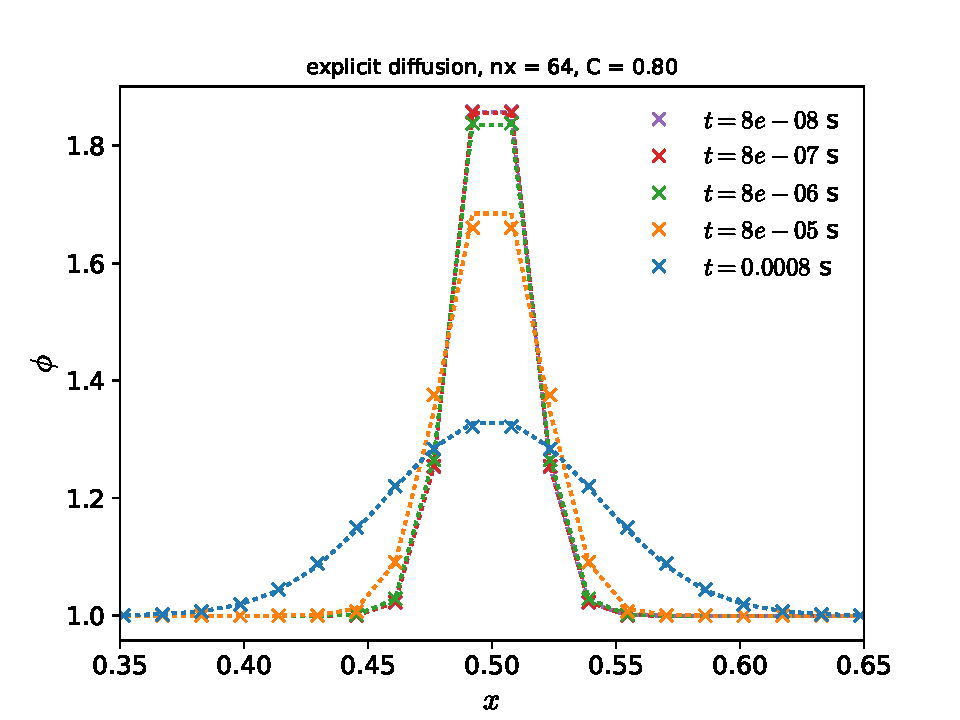
\includegraphics[width=\linewidth]{diff-explicit-64}
\caption[Explicit diffusion of a Gaussian]{\label{fig:diff_explicit}
Diffusion of a Gaussian using the explicit differencing of
Eq.~\ref{eq:diff:explicitdiff} with 64 zones and C = 0.8, shown at
several times.  The dotted line is the analytic
solution.  \\ \hydroexdoit{\href{https://github.com/zingale/hydro_examples/blob/master/diffusion/diffusion_explicit.py}{diffusion\_explicit.py}}}
\end{figure}


\begin{figure}
\centering
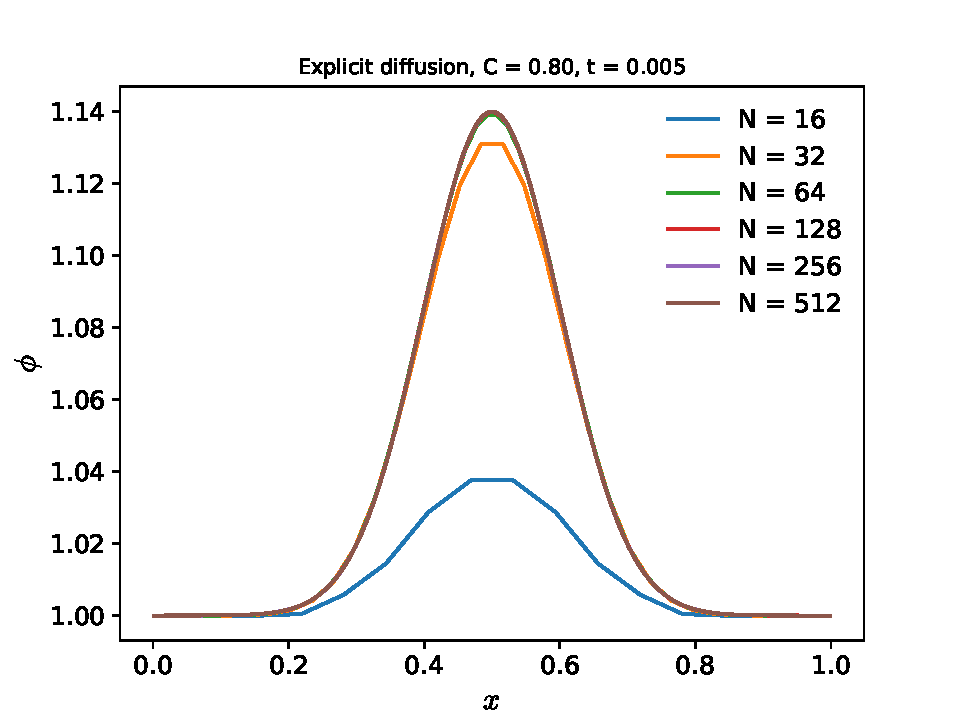
\includegraphics[width=\linewidth]{diffexplicit-res}
\caption[Underresolved explicit diffusion of a Gaussian]{\label{fig:diff_explicit_res}
Diffusion of a Gaussian using the explicit differencing of
Eq.~\ref{eq:diff:explicitdiff} with different resolutions.
several times.  The dotted line is the analytic
solution.  \\ \hydroexdoit{\href{https://github.com/zingale/hydro_examples/blob/master/diffusion/diffusion_explicit.py}{diffusion\_explicit.py}}}
\end{figure}

As with advection, if we exceed the timestep limit ($C > 1$), then
the solution is unstable.  This is shown in Figure~\ref{fig:diff_explicit_bad}.

\begin{figure}
\centering
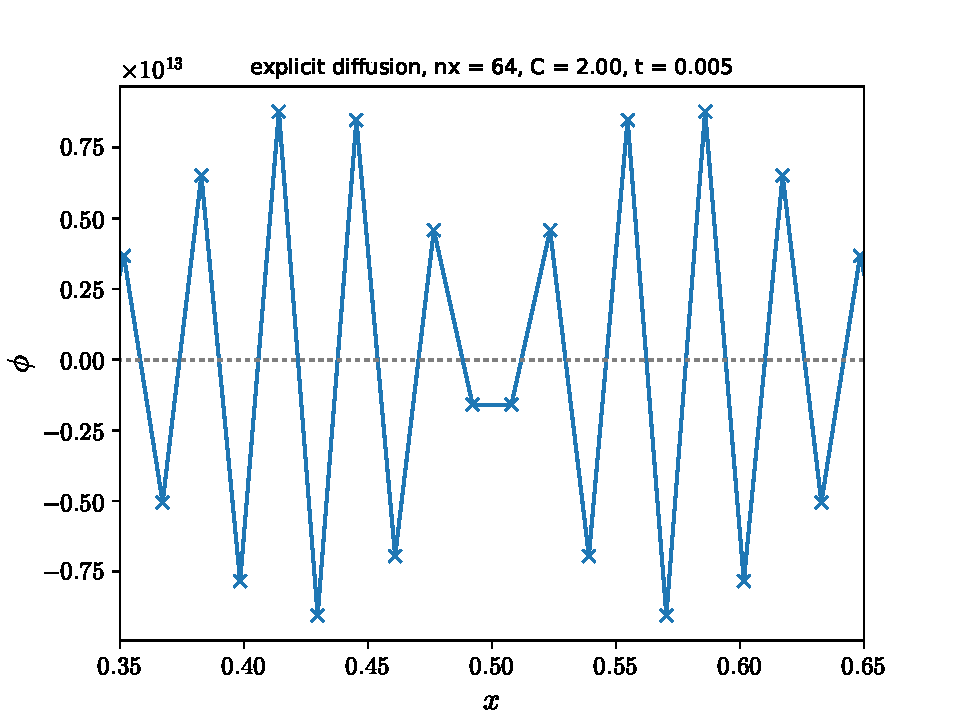
\includegraphics[width=\linewidth]{diff-explicit-64-bad}
\caption[Unstable explicit diffusion]{\label{fig:diff_explicit_bad}
Diffusion of a Gaussian using the explicit differencing of
Eq.~\ref{eq:diff:explicitdiff} with 64 zones, but a timestep
with $C > 1$, showing that the solution is unstable.
 \\ \hydroexdoit{\href{https://github.com/zingale/hydro_examples/blob/master/diffusion/diffusion_explicit.py}{diffusion\_explicit.py}}}
\end{figure}

Our spatial order-of-accuracy is second-order.
Figure~\ref{fig:diffexplicit_converge} shows the error as a function
of number of zones, using the $L_2$ norm of the solution with respect
to the analytic solution.  Notice that at the coarsest resolution
the error is very high---we are not resolving the initial conditions
well enough to have a meaningful solution.

\begin{figure}
\centering
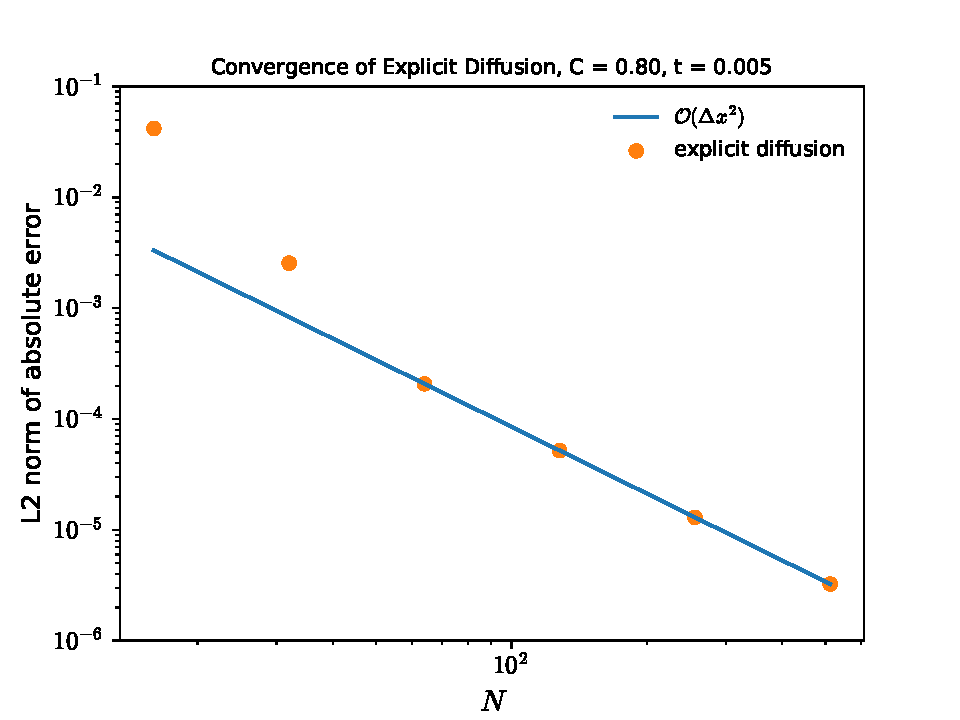
\includegraphics[width=\linewidth]{diffexplicit-converge-0_8}
\caption[Error convergence of explicit diffusion]{\label{fig:diffexplicit_converge}
Error convergence with resolution of the explicit diffusion using the differencing of 
Eq.~\ref{eq:diff:explicitdiff}
 \\ \hydroexdoit{\href{https://github.com/zingale/hydro_examples/blob/master/diffusion/diffusion_explicit.py}{diffusion\_explicit.py}}}
\end{figure}

\section{Implicit with direct solve}

A backward-Euler implicit discretization would be:
\begin{equation}
\frac{\phi_i^{n+1} - \phi_i^n}{\Delta t} = 
  k \frac{\phi_{i+1}^{n+1} - 2\phi_i^{n+1} + \phi_{i-1}^{n+1}}{\Delta x^2}
\end{equation}
This is still first-order in time, but is not restricted by the timestep
constraint (although the timestep will still determine the accuracy).  
Defining:
\begin{equation}
\alpha \equiv k \frac{\Delta t}{\Delta x^2}
\end{equation}
we can write this as:
\begin{equation}
\label{eq:diff:implicit}
-\alpha \phi_{i+1}^{n+1} + (1 + 2\alpha) \phi_{i}^{n+1} - \alpha \phi_{i-1}^{n+1} = \phi_i^n
\end{equation}
This is a set of coupled algebraic equations.  We can write this in
matrix form.  Using a cell-centered grid, we will solve for the values
$[\mathrm{lo},\mathrm{hi}]$.  
The implicit method can use any $C > 0$.

We specify boundary conditions by modifying the stencil
(Eq.~\ref{eq:diff:implicit}) for the updates to $\mathrm{lo}$ and
$\mathrm{hi}$.  For example, Neumann BCs on the left mean:
\begin{equation}
\phi_\mathrm{lo-1} = \phi_\mathrm{lo}
\end{equation}
and substituting this into Eq~\ref{eq:diff:implicit}, the update for the leftmost cell is:
\begin{equation}
 (1 + \alpha) \phi_\mathrm{lo}^{n+1} -\alpha \phi_\mathrm{lo+1}^{n+1}  = 
  \phi_\mathrm{lo}^n
\end{equation}
If we choose Dirichlet BCs on the right ($\phi |_{x=x_l} = A$), then:
\begin{equation}
\phi_\mathrm{hi+1} = 2 A - \phi_\mathrm{hi}
\end{equation}
Substituting this into Eq~\ref{eq:diff:implicit} the update for the rightmost cell is:
\begin{equation}
- \alpha \phi_\mathrm{hi-1}^{n+1} + (1 + 3\alpha) \phi_\mathrm{hi}^{n+1}  =
  \phi_\mathrm{hi}^n + \alpha 2 A
\end{equation}
For all other interior cells, the stencil is unchanged.  The resulting
system can be written in matrix form and appears as a {\em tridiagonal}
matrix.  
\begin{equation}
\renewcommand\arraystretch{1.5}
\left (
\begin{array}{ccccccc}
1+\alpha &   -\alpha &           &        &         &           &          \\
-\alpha  & 1+2\alpha & -\alpha   &        &         &           &          \\
         & -\alpha   & 1+2\alpha & -\alpha&         &           &          \\
         &           & \ddots    & \ddots & \ddots  &           &          \\
         &           &           & \ddots & \ddots  & \ddots    &          \\
         &           &           &        & -\alpha & 1+2\alpha &-\alpha   \\
         &           &           &        &         & -\alpha   &1+3\alpha \\
\end{array}
\right )
\left (
\begin{array}{c}
\phi_\mathrm{lo}^{n+1} \\
\phi_\mathrm{lo+1}^{n+1} \\
\phi_\mathrm{lo+2}^{n+1} \\
\vdots \\
\vdots \\
\phi_\mathrm{hi-1}^{n+1} \\
\phi_\mathrm{hi}^{n+1} \\
\end{array}
\right )
=
\left (
\begin{array}{c}
\phi_\mathrm{lo}^{n} \\
\phi_\mathrm{lo+1}^{n} \\
\phi_\mathrm{lo+2}^{n} \\
\vdots \\
\vdots \\
\phi_\mathrm{hi-1}^{n} \\
\phi_\mathrm{hi}^{n} + \alpha 2 A\\
\end{array}
\right )
\end{equation}
This can be solved by standard matrix operations, using a tridiagonal
solvers (for example).  Notice that the ghost cells do not appear in this
linear system---we are only updating the interior points.

\subsubsection{Crank-Nicolson time discretization}

A second-order in time discretization requires us to center the righthand side in time.  We
do this as:
\begin{equation}
\frac{\phi_i^{n+1} - \phi_i^n}{\Delta t} = 
  \frac{k}{2} \left ( \frac{\phi_{i+1}^{n} - 2\phi_i^{n} + \phi_{i-1}^{n}}{\Delta x^2} +
                      \frac{\phi_{i+1}^{n+1} - 2\phi_i^{n+1} + \phi_{i-1}^{n+1}}{\Delta x^2} \right )
\end{equation}
This time-discretization is called  {\em Crank-Nicolson}.
Again, using $\alpha \equiv k\Delta t / \Delta x^2$, and grouping all the $n+1$ terms on the left
we have:
\begin{equation}
\phi^{n+1}_i - \frac{\alpha}{2} \left ( \phi^{n+1}_{i+1} - 2\phi^{n+1}_i + \phi^{n+1}_{i-1} \right )
  = \phi^n_i + \frac{\alpha}{2} \left ( \phi^{n}_{i+1} - 2\phi^{n}_i + \phi^{n}_{i-1} \right )
\end{equation}
and grouping together the the $n+1$ terms by zone, we have:
\begin{equation}
-\frac{\alpha}{2} \phi^{n+1}_{i+1} + (1 + \alpha)\phi^{n+1}_i - \frac{\alpha}{2} \phi^{n+1}_{i-1}
  = \phi^n_i + \frac{\alpha}{2} \left ( \phi^n_{i+1} - 2 \phi^n_i + \phi^n_{i-1} \right )
\end{equation}

Considering Neumann boundary conditions on the left, we again have
$\phi^{n+1}_\mathrm{lo-1} = \phi^{n+1}_\mathrm{lo}$, and our stencil at the boundary 
becomes
\begin{equation}
-\frac{\alpha}{2} \phi^{n+1}_\mathrm{lo+1} + \left (1 + \frac{\alpha}{2} \right ) \phi^{n+1}_\mathrm{lo} =
    \phi^n_\mathrm{lo} + \frac{\alpha}{2} \left ( \phi^{n}_\mathrm{lo+1} - 2\phi^{n}_\mathrm{lo} + \phi^{n}_\mathrm{lo-1} \right )
\end{equation}

The matrix form of this system is:
\newcommand{\atwo}{\frac{\alpha}{2}}
\begin{equation}
\label{eq:diff:cnmatrix}
\renewcommand\arraystretch{1.5}
\left (
\begin{array}{ccccccc}
1+\atwo &   -\atwo &          &        &        &           &          \\
-\atwo  & 1+\alpha & -\atwo   &        &        &           &          \\
        &   -\atwo & 1+\alpha & -\atwo &        &           &          \\
        &          & \ddots   & \ddots & \ddots &           &          \\
        &          &          & \ddots & \ddots & \ddots    &          \\
        &          &          &        & -\atwo & 1+\alpha  &-\atwo   \\
        &          &          &        &        & -\atwo    &1+\atwo \\
\end{array}
\right )
\left (
\begin{array}{c}
\phi_\mathrm{lo}^{n+1} \\
\phi_\mathrm{lo+1}^{n+1} \\
\phi_\mathrm{lo+2}^{n+1} \\
\vdots \\
\vdots \\
\phi_\mathrm{hi-1}^{n+1} \\
\phi_\mathrm{hi}^{n+1} \\
\end{array}
\right )
=
\left (
\begin{array}{c}
\phi_\mathrm{lo}^{n}  + \frac{k\Delta t}{2} [\nabla^2 \phi]^n_\mathrm{lo}\\
\phi_\mathrm{lo+1}^{n} + \frac{k\Delta t}{2} [\nabla^2 \phi]^n_\mathrm{lo+1} \\
\phi_\mathrm{lo+2}^{n} + \frac{k\Delta t}{2} [\nabla^2 \phi]^n_\mathrm{lo+2}\\
\vdots \\
\vdots \\
\phi_\mathrm{hi-1}^{n} + \frac{k\Delta t}{2} [\nabla^2 \phi]^n_\mathrm{hi-1}\\
\phi_\mathrm{hi}^{n} + \frac{k\Delta t}{2} [\nabla^2 \phi]^n_\mathrm{hi}\\
\end{array}
\right )
\end{equation}

Figure~\ref{fig:diffuse} shows the result of using $\alpha = 0.8$ and $\alpha = 8.0$.  We 
see that they are both stable, but that the smaller timestep is closer to the analytic
solution (especially at early times).

\begin{figure}[t]
\centering
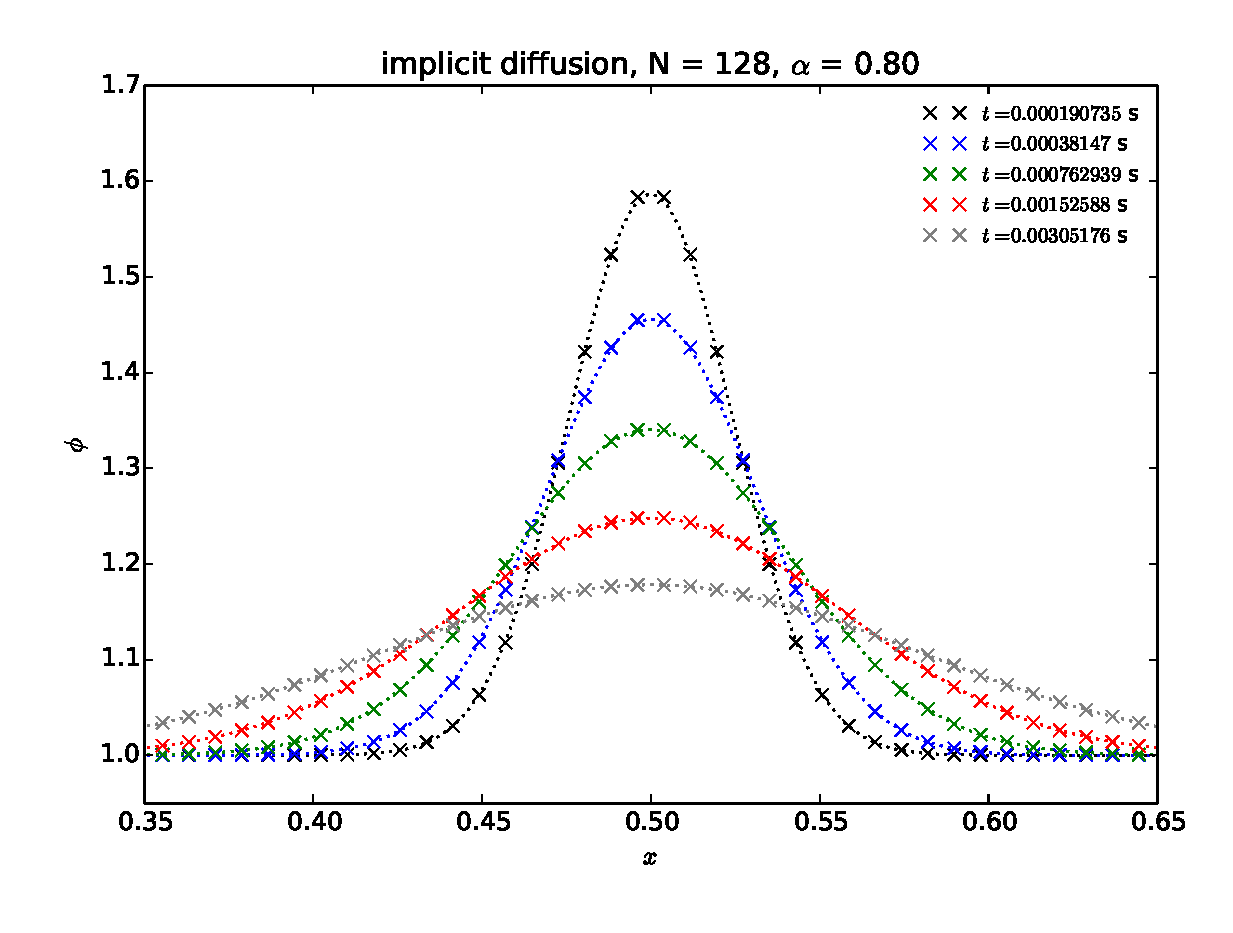
\includegraphics[width=0.75\linewidth]{diff-implicit-128-CFL_0_8}\\
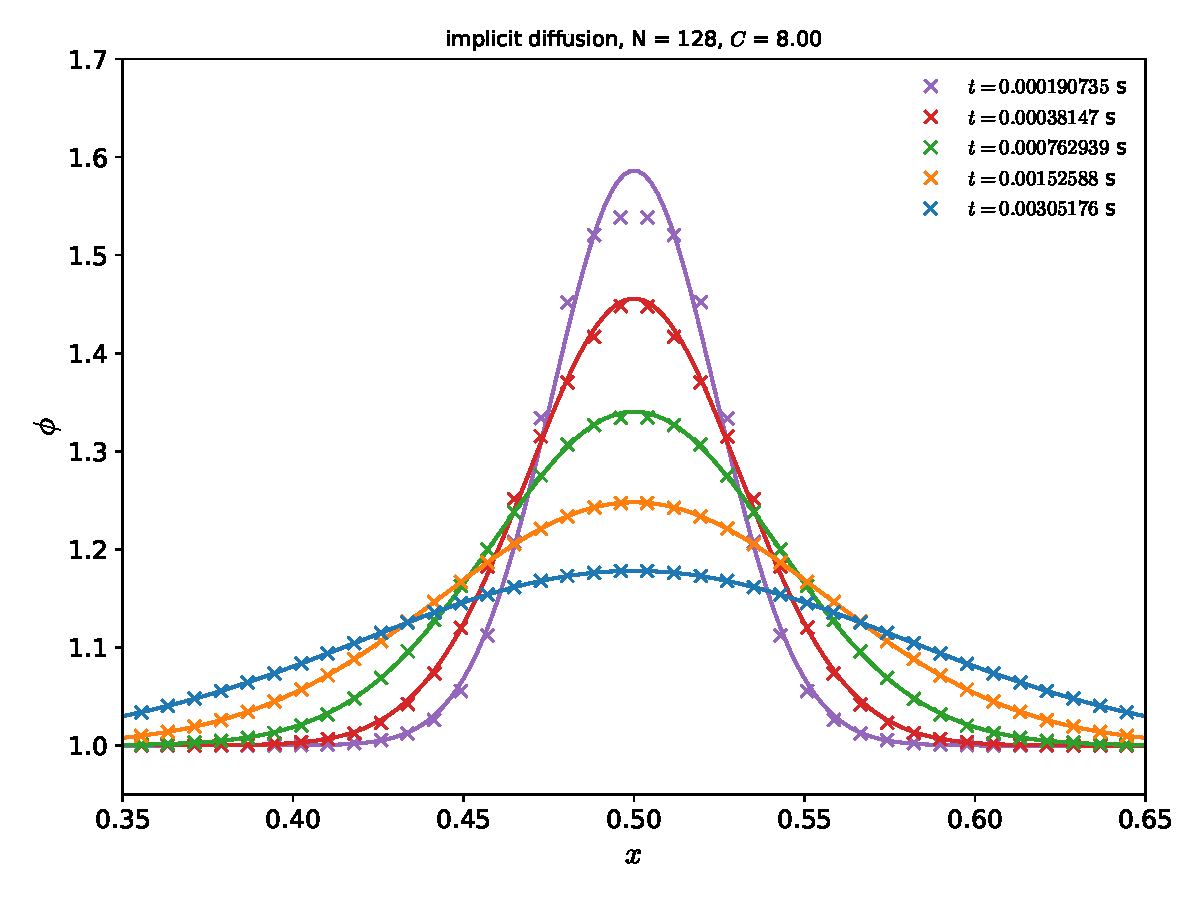
\includegraphics[width=0.75\linewidth]{diff-implicit-128-CFL_8_0}
\caption[Implicit diffusion of a Gaussian]{\label{fig:diffuse}
  Implicit diffusion of a Gaussian (with Crank-Nicolson
  discretization) with $C = 0.8$ and $C = 8.0$.  The exact solution at
  each time is shown as the dotted
  line. \\ \hydroexdoit{\href{https://github.com/zingale/hydro_examples/blob/master/diffusion/diffusion_implicit.py}{diffusion\_implicit.py}}}
\end{figure}

\begin{exercise}[1-d implicit diffusion]
{Write a one-dimensional implicit diffusion solver for the
  domain $[0,1]$ with Neumann boundary conditions at each end and $k = 1$.
  Your solver should use a tridiagonal solver and initialize a matrix like
  that above.  Use a timestep close to the explicit step, a grid with
  N = 128 zones.

  Use a Gaussian for your initial conditions (as you did for the 
  explicit problem.}
\end{exercise}


\section{Implicit multi-dimensional diffusion via multigrid}

Instead of doing a direct solve of the matrix form of the system, we 
can use multigrid techniques.  Consider the Crank-Nicolson system we just 
looked at:
\begin{equation}
\frac{\phi^{n+1}_i - \phi^n_i}{\Delta t} = 
   \frac{1}{2} \left ( k \nabla^2 \phi^n_i + k \nabla^2 \phi^{n+1}_i \right )
\end{equation}
Grouping all the 
$n+1$ terms on the left, we find:
\begin{equation}
\phi^{n+1}_i - \frac{\Delta t}{2} k \nabla^2 \phi^{n+1}_i = 
    \phi^n_i + \frac{\Delta t}{2} k \nabla^2 \phi^n_i
\end{equation}
This is in the form of a constant-coefficient Helmholtz equation,
\begin{equation}
\label{eq:diff:helmholtz}
(\alpha - \beta \nabla^2) \phi^{n+1} = f
\end{equation}
with
\begin{eqnarray}
\alpha &=& 1 \\
\beta &=& \frac{\Delta t}{2} k \\
f &=& \phi^n + \frac{\Delta t}{2} k \nabla^2 \phi^n
\end{eqnarray}
This can be solved using multigrid techniques with a Helmholtz
operator.  The same boundary conditions discussed in
Chapter~\ref{ch:multigrid} apply here.  The main difference between
the multigrid technique for the Poisson problem and the Helmholtz
problem is the form of the smoother.  In 1-d, we discretize
Eq.~\ref{eq:diff:helmholtz} with a second-order difference expression
for the second derivative, and isolate $\phi_i$, giving a smoothing
operation of the form:
\begin{equation}
\phi_{i} \leftarrow
 \left .    \left ( f_{i} + \frac{\beta}{\Delta x^2} [\phi_{i+1}
                             + \phi_{i-1}] \right ) \middle / 
\left ( \alpha + \frac{2 \beta}{\Delta x^2}  \right )  \right .
\end{equation}

Note: when using multigrid, you do not need to actually construct the
matrix.  This is usually the most efficient way to implement diffusion
in a multi-dimensional simulation code, especially when distributing
the grid across parallel processors.  Since the discretization is the
same as the direct matrix solve, Eq.~\ref{eq:diff:cnmatrix}, the
result will be exactly the same (to the tolerance of the multigrid
solver).


\subsection{Convergence}

One needs to be careful with the Crank-Nicolson discretization.  If
the initial data is under-resolved and you are taking a big timestep
($C \gg 1$), then the method can be unstable.
Figure~\ref{fig:diff:cnunstable} shows such a case for the Gaussian
diffusion with Crank-Nicolson discretization and 64 zones with $C =
10$.  For this reason, simulation codes often drop down to the
simple backwards difference time-discretization for implicit diffusion
of under-resolved flows.

\begin{figure}
\centering
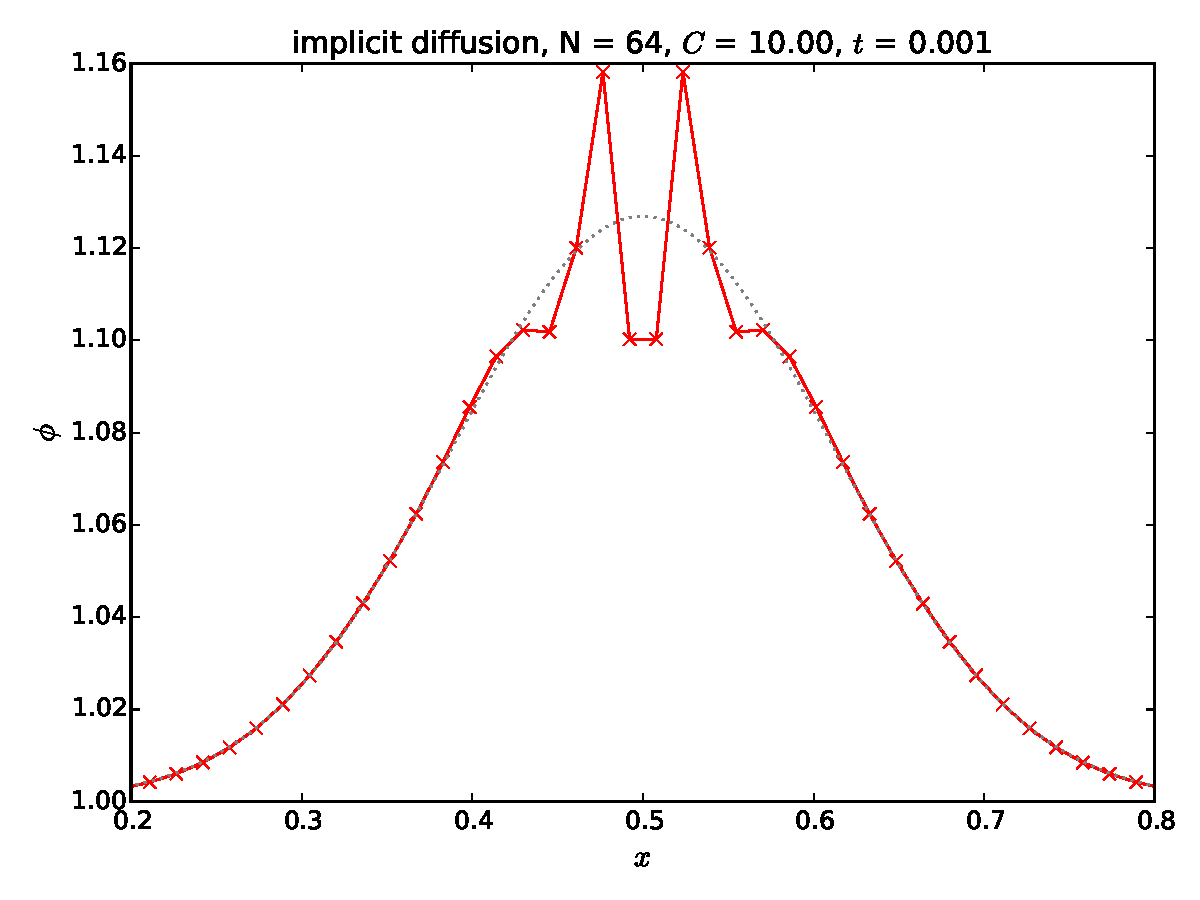
\includegraphics[width=\linewidth]{diff-implicit-64-CFL_10_0}
\caption[Under-resolved Crank-Nicolson diffusion]
{\label{fig:diff:cnunstable} Crank-Nicolson diffusion of a Gaussian
on under-resolved initial data with a large timestep.  Here we use
$64$ zones and $C= 10$.}
\end{figure}


\begin{figure}
\centering
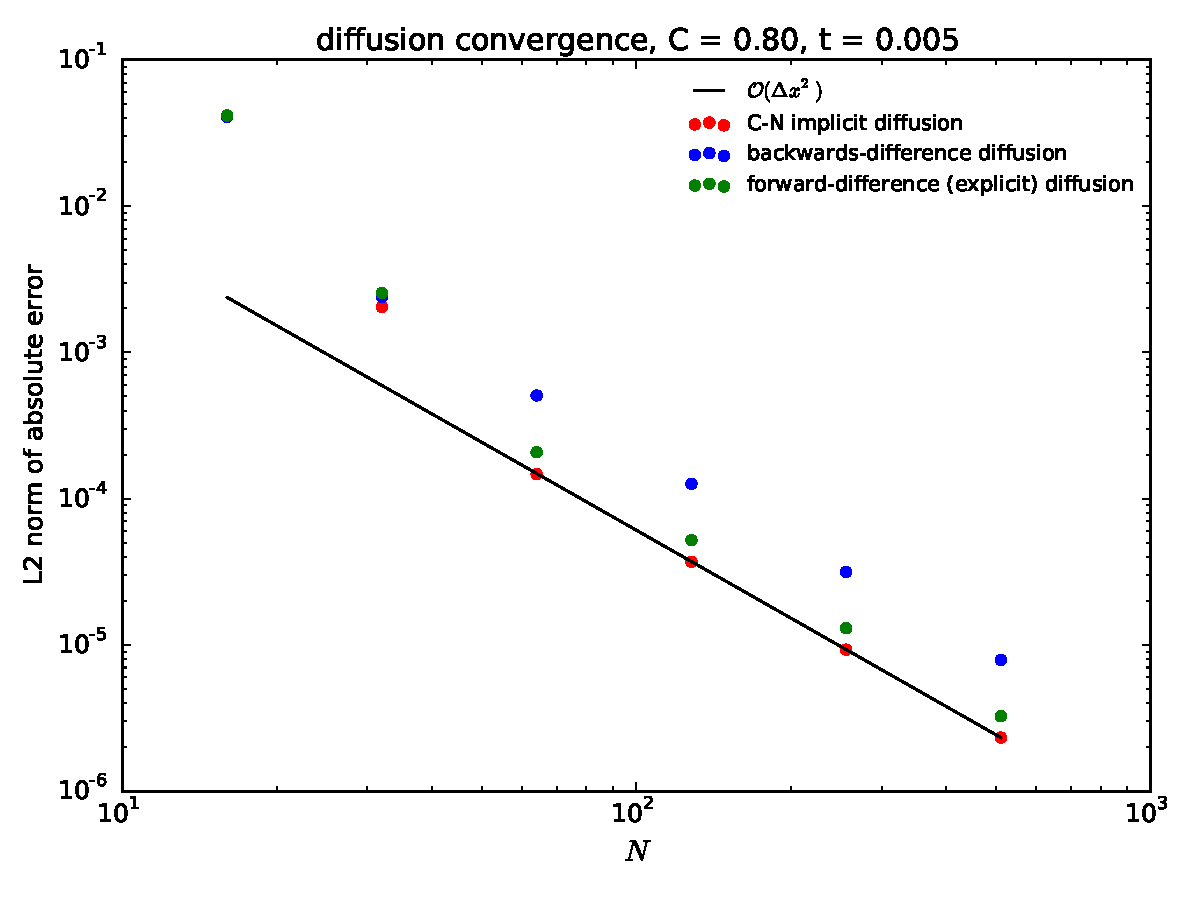
\includegraphics[width=0.75\linewidth]{diffimplicit-converge-0_8} \\
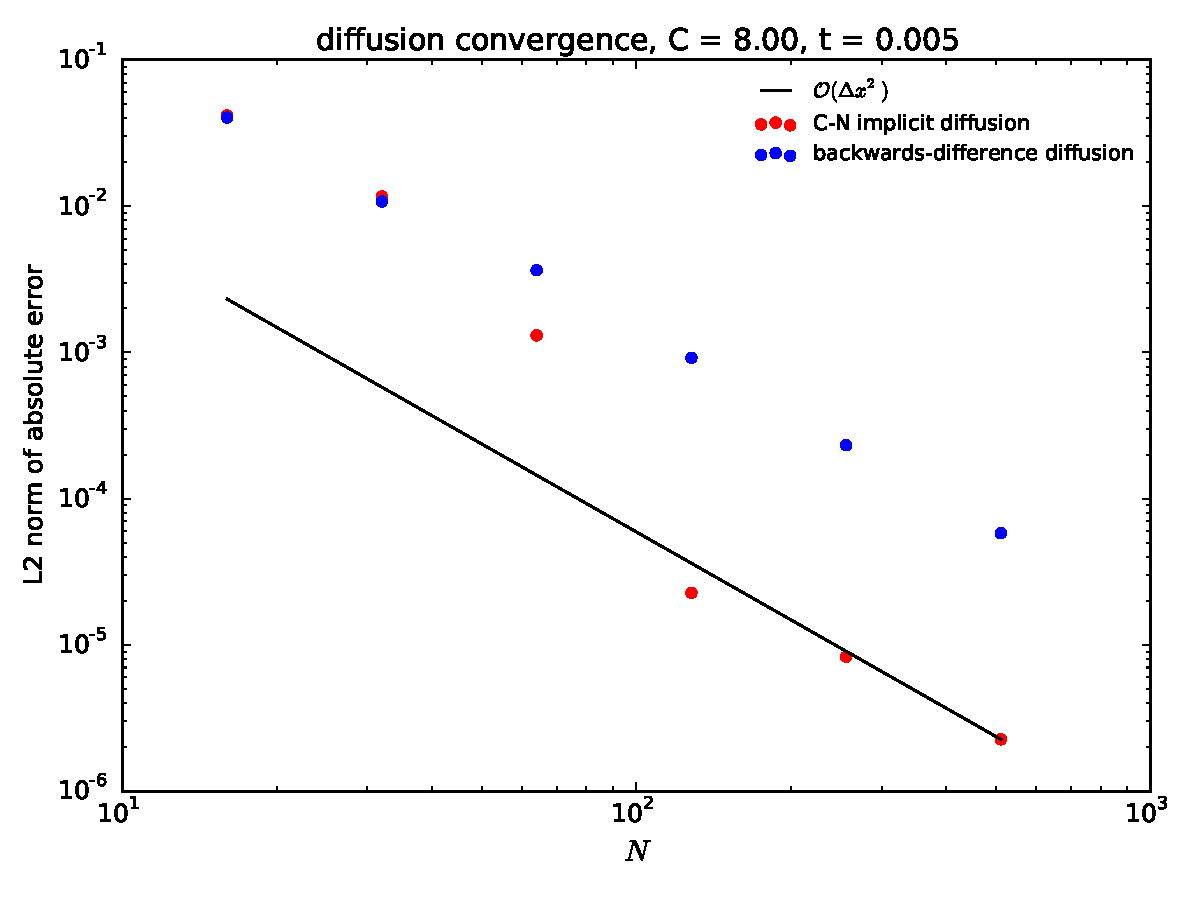
\includegraphics[width=0.75\linewidth]{diffimplicit-converge-8_0} 
\caption[Convergence of diffusion methods]
{\label{fig:diff:convergence} Convergence of the explicit, backward-difference,
and Crank-Nicolson diffusion methods for $C = 0.8$ (top) and $C = 8.0$ (bottom).
For the latter case, the explicit method is not valid and is not shown.
We see that the Crank-Nicolson method has the lowest error, and when resolving
the data, has second-order convergence.\\
\hydroexdoit{\href{https://github.com/zingale/hydro_examples/blob/master/diffusion/diff_converge.py}{diff\_converge.py}}}
\end{figure}

\section{Going further}

\begin{itemize}

\item {\em Non-constant conductivity}: for the case where $k = k(x)$,
  we discretize as:
  \begin{equation}
  \frac{\phi_i^{n+1} - \phi_i^n}{\Delta t} = 
        \frac{ \{ k \nabla \phi \}_{i+1/2} -
               \{ k \nabla \phi \}_{i-1/2}}{\Delta x}
  \end{equation}
 Here we need the values of $k$ at the interfaces, $k_{i-1/2}$ and
 $k_{i+1/2}$.  We can get these from the cell-centered values in a
 variety of ways including straight-averaging:
 \begin{equation}
 k_{i+1/2} = \frac{1}{2} (k_i + k_{i+1})
 \end{equation}
 or averaging the inverses:
 \begin{equation}
 \frac{1}{k_{i+1/2}} = \frac{1}{2} \left (\frac{1}{k_i} + \frac{1}{k_{i+1}} \right )
 \end{equation}
 
\item {\em State-dependent transport coefficients}: many times the
  transport coefficients themselves depend on the quantity being
  diffused:
  \begin{equation}
  \frac{\phi_i^{n+1} - \phi_i^n}{\Delta t} = 
        \frac{1}{2} \left \{
               \nabla \cdot [ k(\phi^n) \nabla \phi^n ]_i +
               \nabla \cdot [ k(\phi^{n+1}) \nabla \phi^{n+1} ]_i 
               \right \}
  \end{equation}
  (for example, with thermal diffusion, the conductivity can
  be temperature dependent).  In this case, we can achieve second-order
  accuracy by doing a predictor-corrector.  First we diffuse with
  the transport coefficients evaluated at the old time, giving a provisional
  state, $\phi^\star$:
  \begin{equation}
  \frac{\phi_i^\star - \phi_i^n}{\Delta t} = 
        \frac{1}{2} \left \{
               \nabla \cdot [ k(\phi^n) \nabla \phi^n ] +
               \nabla \cdot [ k(\phi^n) \nabla \phi^\star ] 
               \right \}
  \end{equation}
  Then we redo the diffusion, evaluating $k$ with $\phi^\star$ to
  center the righthand side in time, giving the new state, $\phi^{n+1}$:
  \begin{equation}
  \frac{\phi_i^{n+1} - \phi_i^n}{\Delta t} = 
        \frac{1}{2} \left \{
               \nabla \cdot [ k(\phi^n) \nabla \phi^n ] +
               \nabla \cdot [ k(\phi^\star) \nabla \phi^{n+1} ] 
               \right \}
  \end{equation}
  This is the approach used, for example, in \cite{SNpaper}.


\item {\em Temperature diffusion in energy equation}: Often we find
 diffusion represented as one of many physical processes in a single
 equation.  For example, consider the internal energy equation with
 both reactions and diffusion:
 \begin{equation}
 \rho\frac{\partial e}{\partial t} + \rho U \cdot \nabla e + p \nabla \cdot U = \nabla \cdot k \nabla T + \rho S
 \end{equation}
 This can be solved via an explicit-implicit discretization.  First
 the advection terms are computed as:
 \begin{equation}
 A = \rho U \cdot \nabla e + p \nabla \cdot U
 \end{equation}
 Then the advective-diffusive part is solved implicitly.  Expressing
 $e = e(\rho, T)$, and using the chain rule,
 \begin{equation}
   \nabla e = e_T \nabla T + e_\rho \nabla \rho
 \end{equation}
 where $e_T = \partial e / \partial T |_\rho \equiv c_v$ is the
 specific heat at constant volume and $e_\rho = \partial e / \partial
 \rho |_T$.  Rewriting, we have:
 \begin{equation}
 \nabla T = (\nabla e - e_\rho \nabla \rho)/c_v
 \end{equation}
  and then
 \begin{equation}
 \rho \frac{\partial e}{\partial t} = \nabla \cdot (k/c_v) \nabla e - \nabla \cdot (k e_\rho/c_v) \nabla \rho -A + \rho S
 \end{equation}
 This is now a diffusion equation for $e$, which can be solved by the
 techniques described above.  This is discussed, for example, in
 \cite{SNpaper,malone:2011}.
\end{itemize}

